\documentclass[a4paper,12pt]{article}
\usepackage{times}
\usepackage[francais]{babel}
\usepackage[utf8x]{inputenc}
\usepackage[T1]{fontenc}
\usepackage{amsmath}
\usepackage{amssymb}
\usepackage{graphicx}
\usepackage{pdfpages}
\usepackage{pdflscape}
\usepackage{listings}
\usepackage{longtable}
\lstset{literate=
{é}{{\'e}}1
{è}{{\`e}}1
{ê}{{\^e}}1
{à}{{\`a}}1
{â}{{\^a}}1
}
\lstset{language=C++,
                basicstyle=\footnotesize,
                keywordstyle=\footnotesize\color{blue},
                otherkeywords={override,nullptr}
}
\definecolor{orange}{rgb}{0.8,0.4,0.0}
\definecolor{darkblue}{rgb}{0.0,0.0,0.6}
\definecolor{cyan}{rgb}{0.0,0.6,0.6}
\lstdefinelanguage{JSON}
{
  basicstyle=\normalsize,
  columns=fullflexible,
  showstringspaces=false,
  commentstyle=\color{gray}\upshape,
  morestring=[b]",
  morestring=[s]{>}{<},
  morecomment=[s]{<?}{?>},
  stringstyle=\color{orange},
  identifierstyle=\color{darkblue},
  keywordstyle=\color{blue},
  morekeywords={string,number,array,object}% list your attributes here
}

\sloppy

\setlength{\topmargin}{0cm}
\setlength{\headsep}{0.in}
\setlength{\headheight}{0.in}
\setlength{\evensidemargin}{0cm}
\setlength{\oddsidemargin}{-1cm}
\textwidth 18cm
\textheight 25cm

\begin{document}

\thispagestyle{empty}

\begin{titlepage}

\vspace*{2cm}

\begin{center}\textbf{\Huge Projet Logiciel Transversal}\end{center}{\Large \par}

\begin{center}\textbf{\large WANG Zhao BENMIRA Eltadj PRADINES Louis}\end{center}{\large \par}

\vspace{2cm}

\begin{figure}[h]
\begin{center}
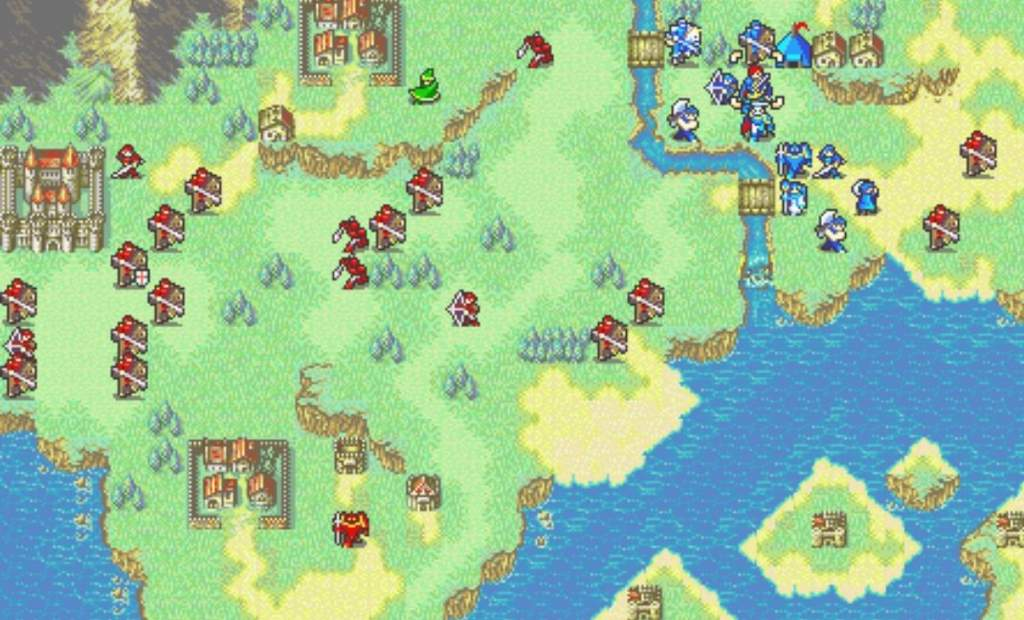
\includegraphics[width=\textwidth]{exemple.jpg}
\caption{\label{pacmangame}Exemple du jeu}
\end{center}
\end{figure}

\clearpage

{\small
\tableofcontents
}

\end{titlepage}

\clearpage
\section{Présentation Générale}

\subsection{Archétype}

L'objectif de ce projet est de réaliser un tactical RPG à la Fire Emblem, un exemple est proposé à la figure 1. Un tactical RPG est un jeu de rôle tactique. Dans ce genre de jeu vidéo, le gameplay est basé sur les décisions tactiques que le joueur doit prendre au cours des combats. Le joueur doit utiliser ses personnages pour éliminer tous les personnages ennemis du plateau, chaque personnage possède comme dans un RPG traditionnel un niveau et des statistiques qui définissent sa puissance. 

\subsection{Règles du jeu}
\subsubsection{Présentation des règles}
Pour gagner la partie il faut tuer tous les personnages de l'ennemi (chaque joueur a 5 personnages). On joue au tour par tour, un tour est fini lorsque tous les personnages d’un joueur ont joué. 
Un personnage doit faire ces actions dans son tour :
\begin{enumerate}
  \item se déplacer de [0 cases, maximum de distance parcourable]
  \item attaquer si il y a un ennemi dans sa portée d’attaque xor utiliser une potion xor attendre 
\end{enumerate}
Chaque personnage possède des points de mouvement qu’il régénère au début de chaque tour, se déplacer sur une case consomme normalement 1 point de mouvement (ça dépend du type de case traversée). Lorsqu’il n’a plus de points de mouvements, un personnage ne peut plus se déplacer.
\subsubsection{Plateau}
Le plateau fait 64x64 cases, chaque cases possède des particularités
\begin{figure}[ht]
\begin{center}
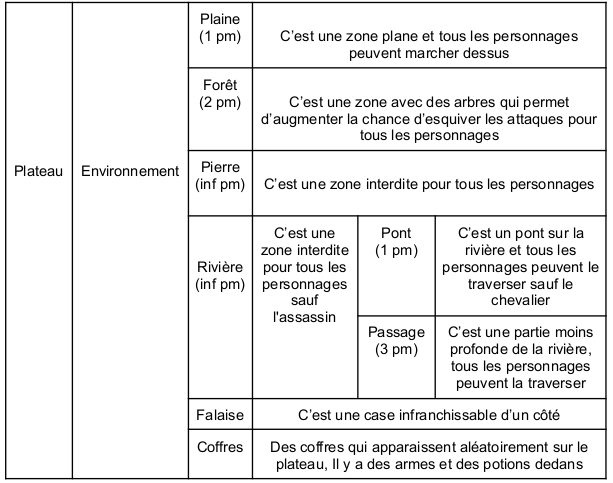
\includegraphics[width=0.7\textwidth]{tableauplateau.png}
\end{center}
\end{figure}
\newpage
\subsubsection{Saisons}
Il y a quatre saisons à la fin de chaque tour (lorsque les 2 joueurs ont joué) la saison change. Chaque saison donne des bonus généraux à tous les personnages, des bonus spécifiques aux personnages qui sont reliés à celle-ci et des malus aux personnages qui sont reliés à la saison opposée. L’ordre des saisons est le suivant: Printemps → Été → Automne → Hiver
\begin{figure}[ht]
\begin{center}
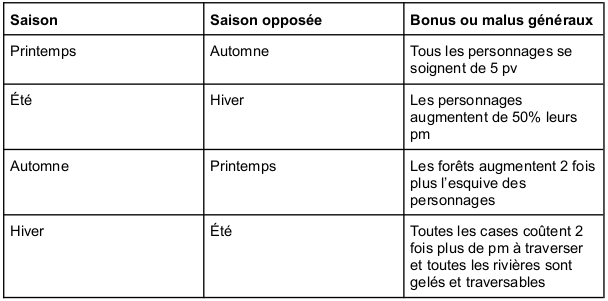
\includegraphics[width=0.7\textwidth]{tableausaison.png}
\end{center}
\end{figure}
\subsubsection{Personnages}
Chaque joueur dispose de 5 personnages ( Assassin,mage,chevalier,archer et combattant ). Ces personnages possèdent des armes et des spécificités liées à la saison auxquelles ils sont reliés:
\begin{figure}[ht]
\begin{center}
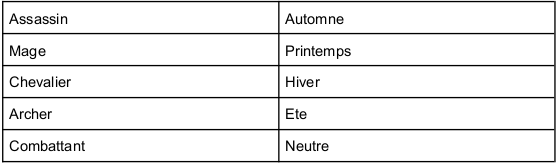
\includegraphics[width=0.7\textwidth]{tableaupersonnages.png}
\end{center}
\end{figure}
\paragraph{}
Lorsque la saison d’un personnage est effective, ce joueur possède des bonus  qui améliorent ses attaques et sa défense ainsi que ses déplacements.
Chaque personnage possède ses propres armes et bonus lié à sa particularité: 
\paragraph{}
L' assassin: L'assassin possède une dague, il traverse les cases rivières, et un bonus est appliqué à son attaque lorsqu'il attaque par derrière. En automne sa technique est multipliée par 2. Au printemps sa technique est divisée par deux.
\paragraph{}
Le Mage: Le mage utilise magie, il peut apporter des soins. 
Au printemps le mage a la capacité de ressusciter le dernier personnage tué de son équipe. En hiver le mage perd ses pouvoirs de soin, il peut donc plus soigner aucun personnage. 
\paragraph{}
Le chevalier: Le chevalier possède pour arme une épée, c'est un cavalier il a donc un grand nombre de points de déplacement. Il a pour particularité de pouvoir se déplacer après avoir attaqué (s' il lui reste des points de mouvements) mais il a pour malus de ne pas pouvoir traverser les ponts. En hiver le chevalier à la capacité d’augmenter sa défense. En été, la défense du chevalier est divisée par deux . 
\paragraph{}
Archer: l’archer possède pour arme un arc et des flèches, il a pour spécificité de pouvoir augmenter sa portée d'attaque lorsqu'il est sur une case montagne. 
En été sa portée augmente mais en hiver elle baisse.  
\paragraph{}
Combattant: Le combattant  a pour arme une lance par défaut au début du jeu mais il a la capacité contrairement aux autres personnages de pouvoir porter toutes les armes possible.  Il est considéré comme un personnage ‘neutre ‘ il n’a donc pas de spécificité lié aux saisons.
Le combattant possède un bonus qui lui permet d’obtenir deux fois plus d’armes à l’ouverture d’un coffre.

\subsubsection{Statistiques}
Chaque personnage possède des statistiques qui augmentent aléatoirement dès qu’il gagne un niveau
\begin{figure}[ht]
\begin{center}
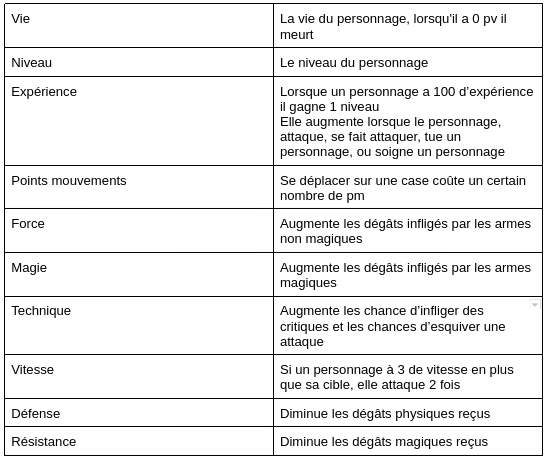
\includegraphics[width=0.7\textwidth]{tableaustats.png}
\end{center}
\end{figure}
\newpage
\subsubsection{Objets}
\begin{figure}[ht]
\begin{center}
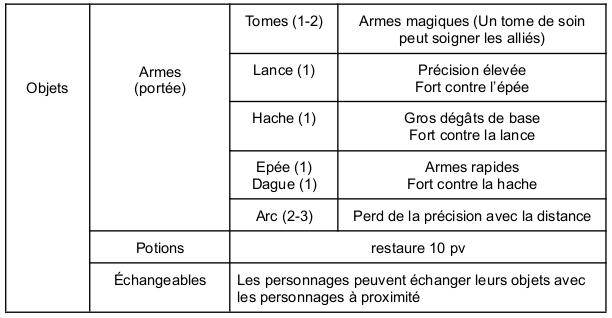
\includegraphics[width=0.7\textwidth]{tableauobjets.png}
\end{center}
\end{figure}
\subsection{Ressources}
On a besoin de textures pour les cases, une case est un carré de 128 pixels. Les textures des cases de type herbe changent de couleur en fonction des saisons
Chaque personnage a un modèle carré de 128 pixels qui le représente sur le plateau et un portrait plus détaillé qui le représente dans l'écran de statistique, dans les dialogues,...
\begin{figure}[ht]
\begin{center}
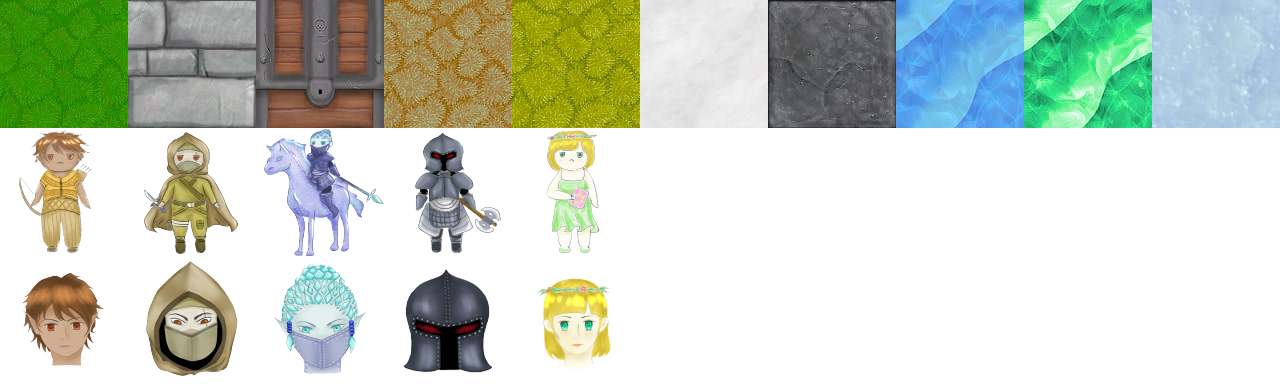
\includegraphics[width=0.7\textwidth]{textures.png}
\caption{\label{pacmangame}Les textures du jeu}
\end{center}
\end{figure}
\newpage
La police du jeu est la suivante 
\begin{figure}[ht]
\begin{center}
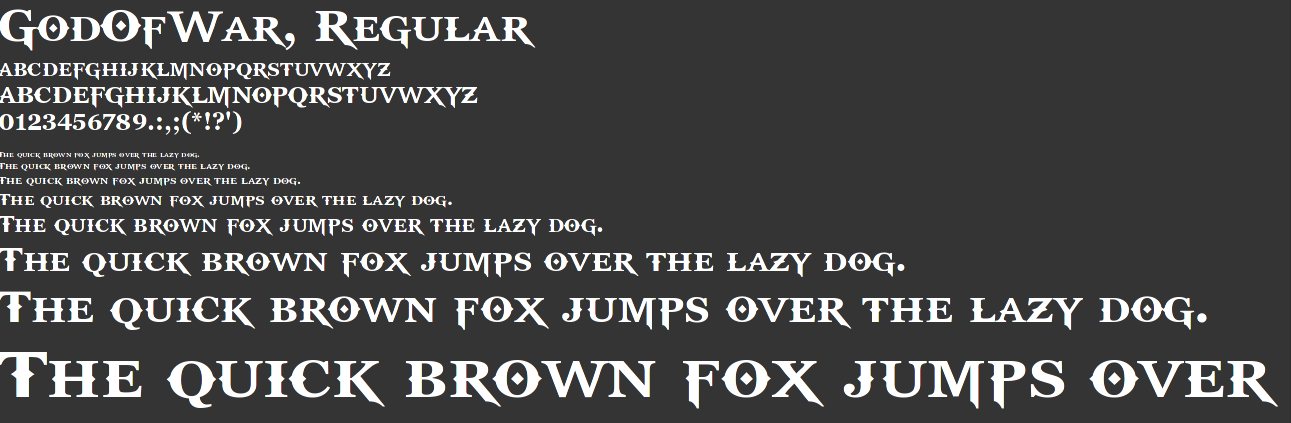
\includegraphics[width=0.7\textwidth]{ressource_police.png}
\caption{\label{pacmangame}La police du jeu}
\end{center}
\end{figure}
\clearpage
\section{Description et conception des états}

\subsection{Description des états}


\subsection{Conception Logiciel}


%\begin{landscape}
%\begin{figure}[p]
%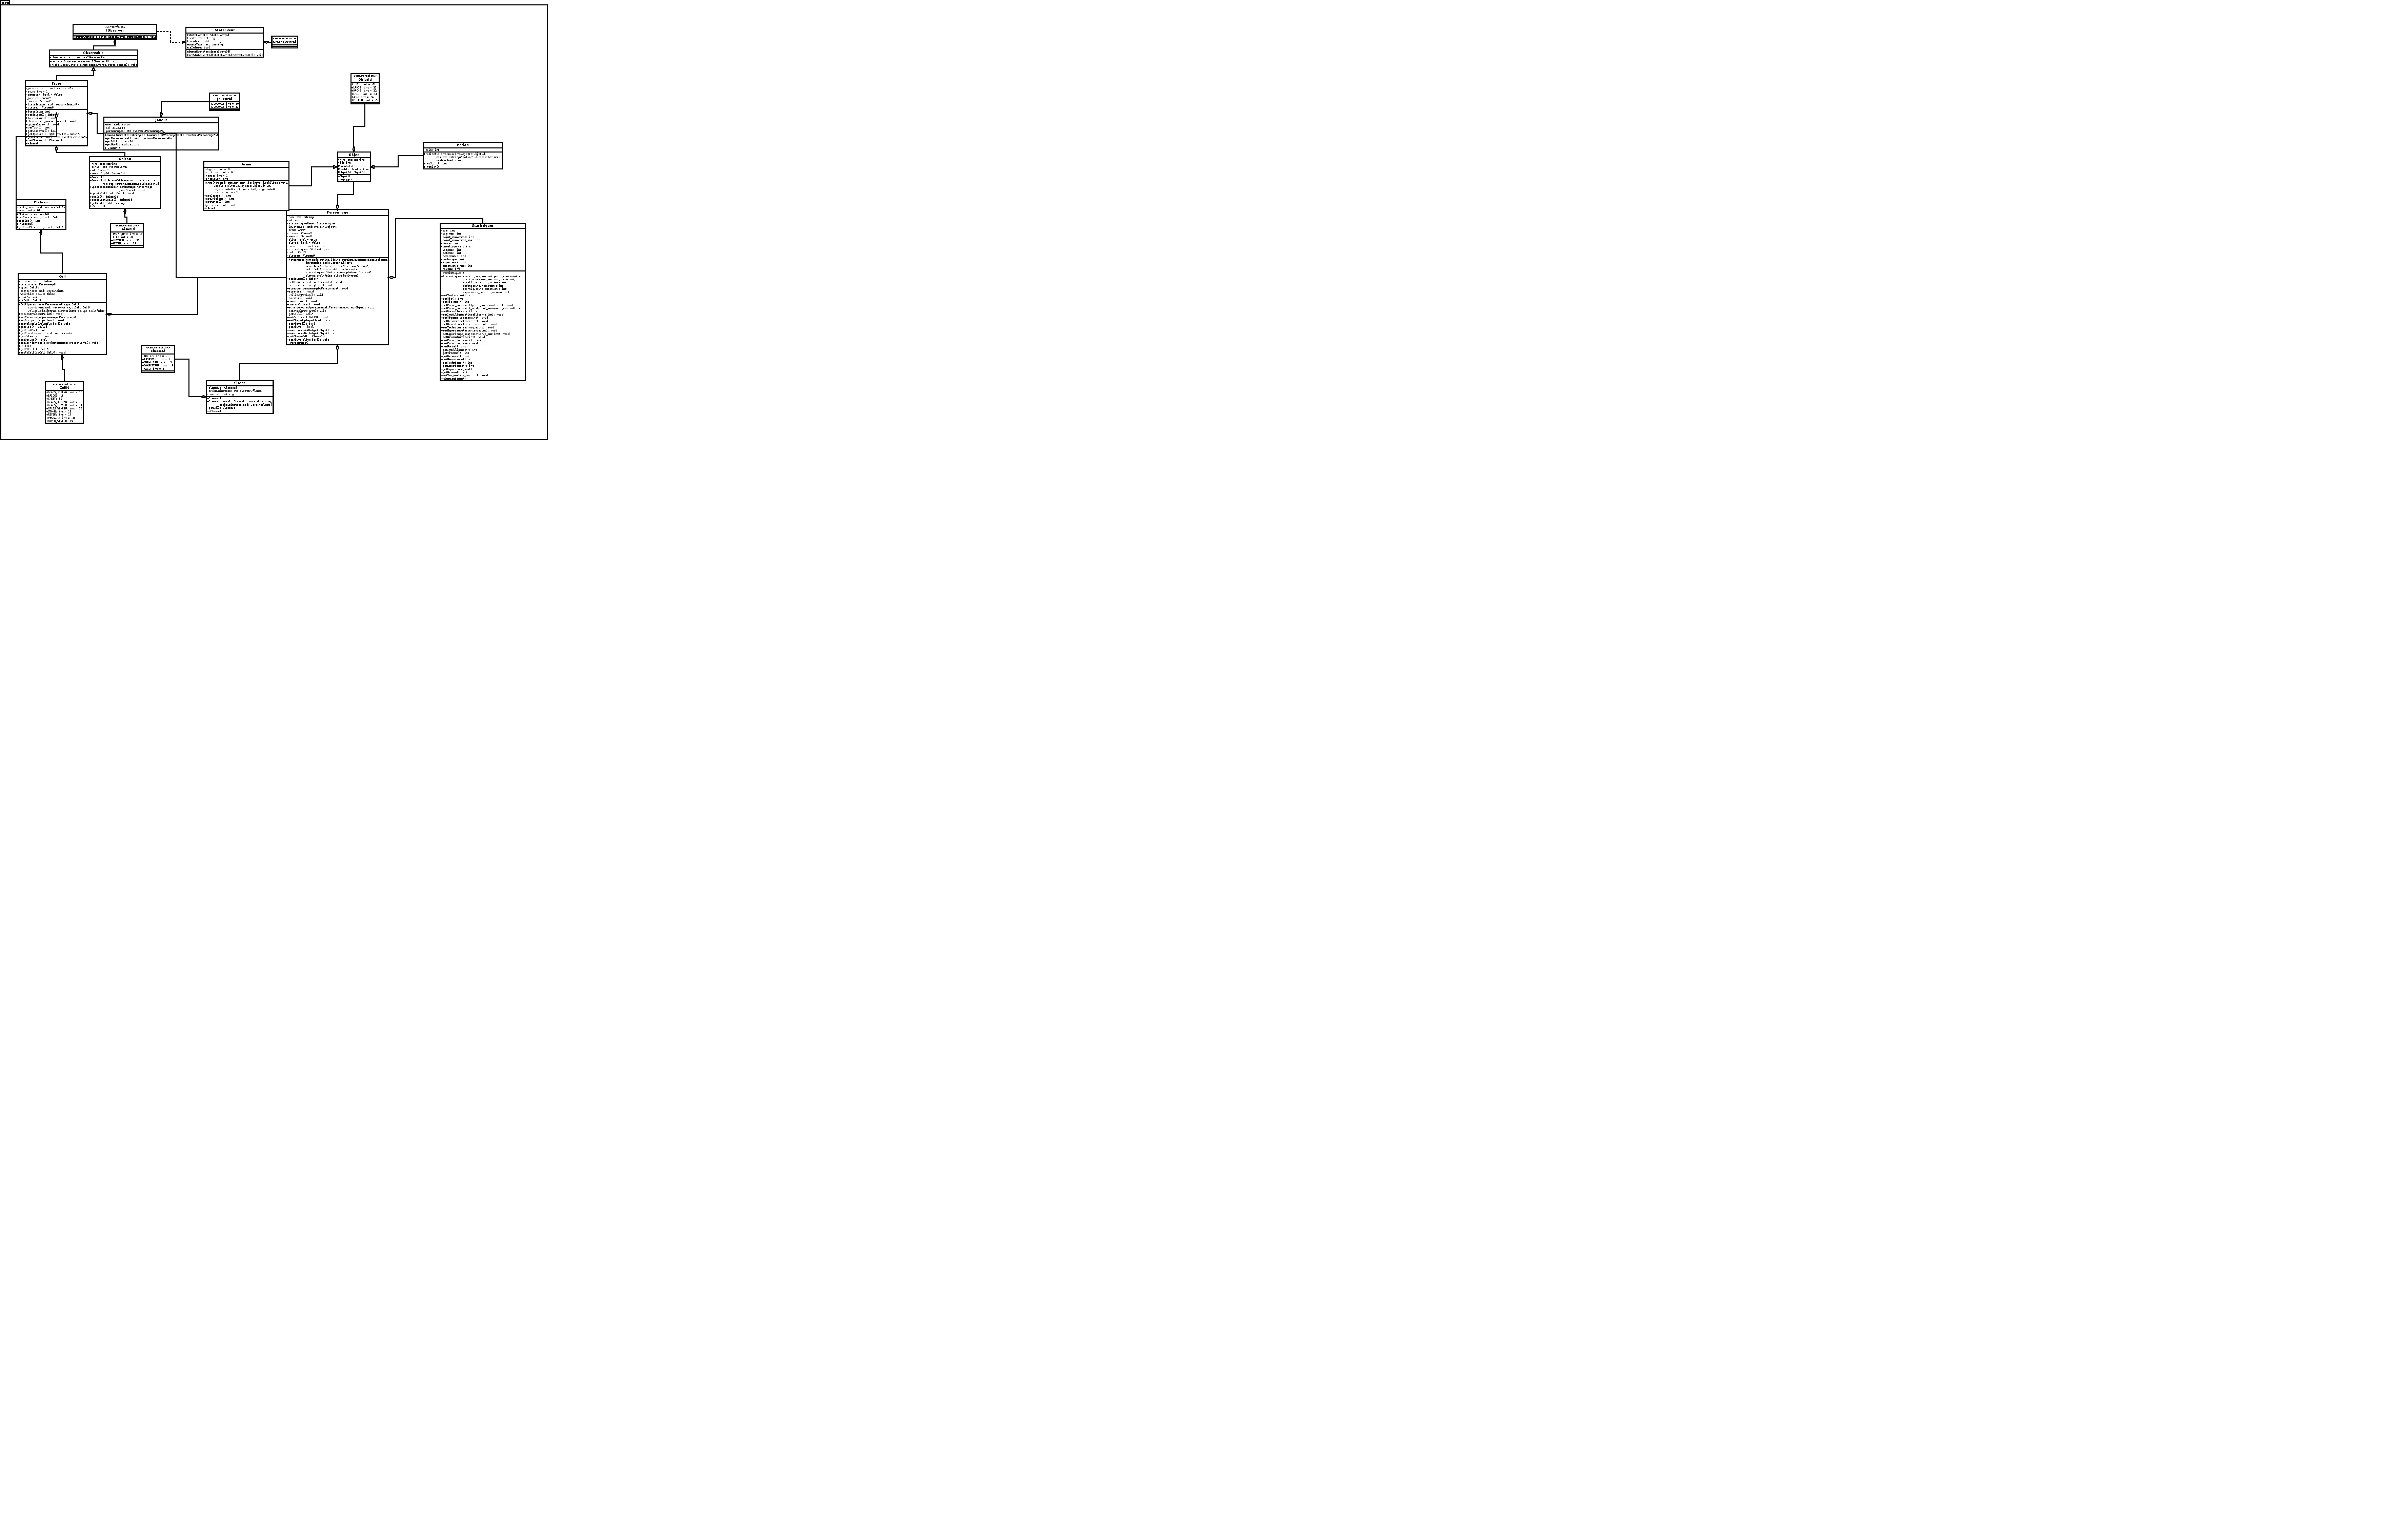
\includegraphics[width=0.9\paperheight]{state.pdf}
%\caption{\label{uml:state}Diagramme des classes d'état.} 
%\end{figure}
%\end{landscape}

\clearpage
\section{Rendu: Stratégie et Conception}

\subsection{Stratégie de rendu d'un état}


\subsection{Conception logiciel}

%\begin{landscape}
%\begin{figure}[p]
%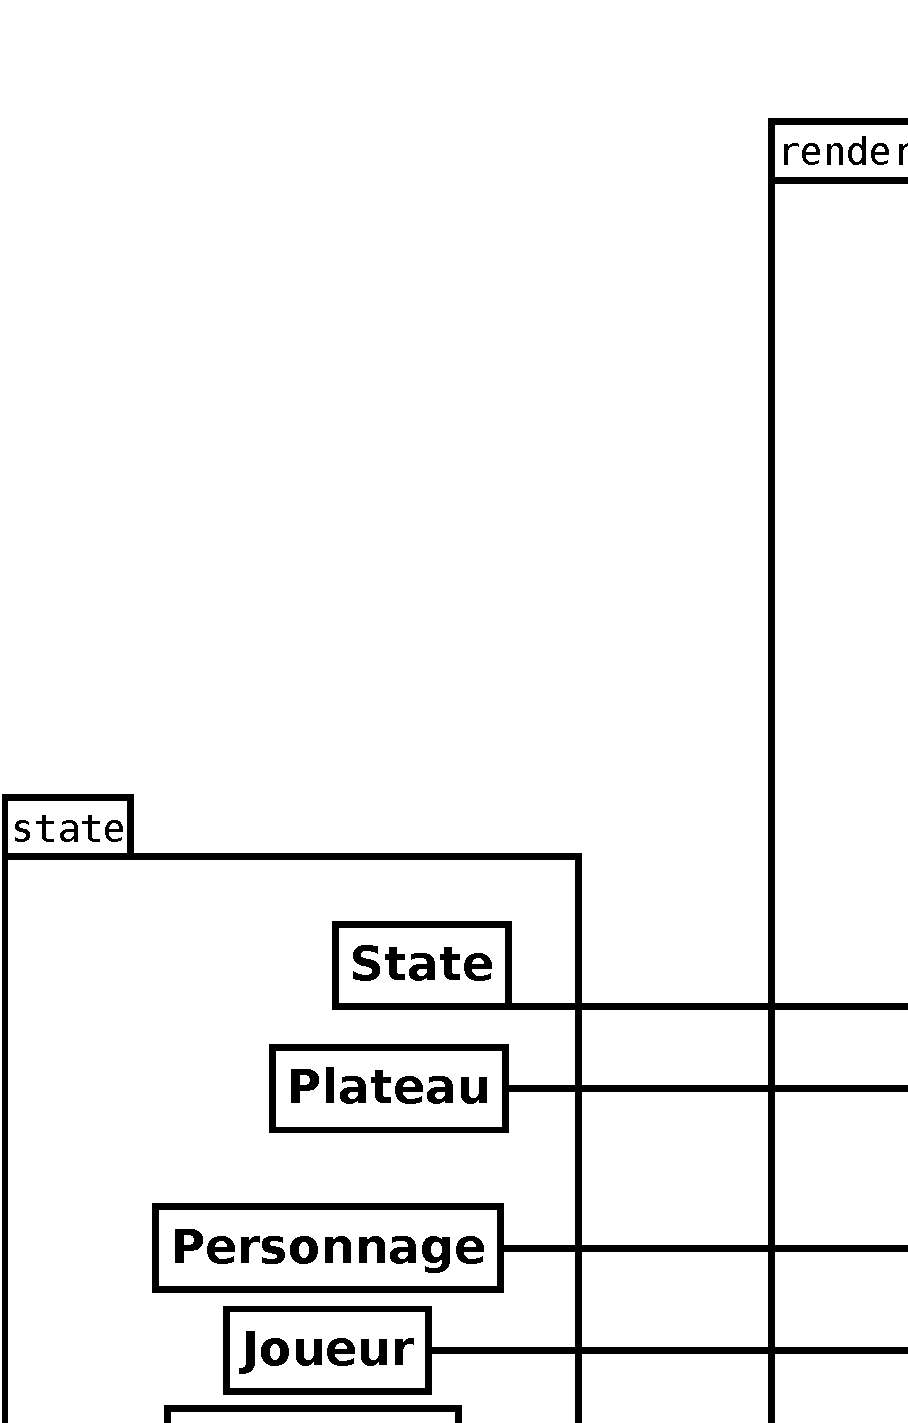
\includegraphics[width=0.9\paperheight]{render.pdf}
%\caption{\label{uml:render}Diagramme des classes de rendu.} 
%\end{figure}
%\end{landscape}

\clearpage
\section{Règles de changement d'états et moteur de jeu}

\subsection{Règles}

\clearpage
\subsection{Conception logiciel}


%\begin{landscape}
%\begin{figure}[p]
%\includegraphics[width=0.9\paperheight]{engine.pdf}
%\caption{\label{uml:engine}Diagramme des classes de moteur de jeu.} 
%\end{figure}
%\end{landscape}


\section{Intelligence Artificielle}

\subsection{Stratégies}

\clearpage
\subsection{Conception logiciel}


%\begin{landscape}
%\begin{figure}[p]
%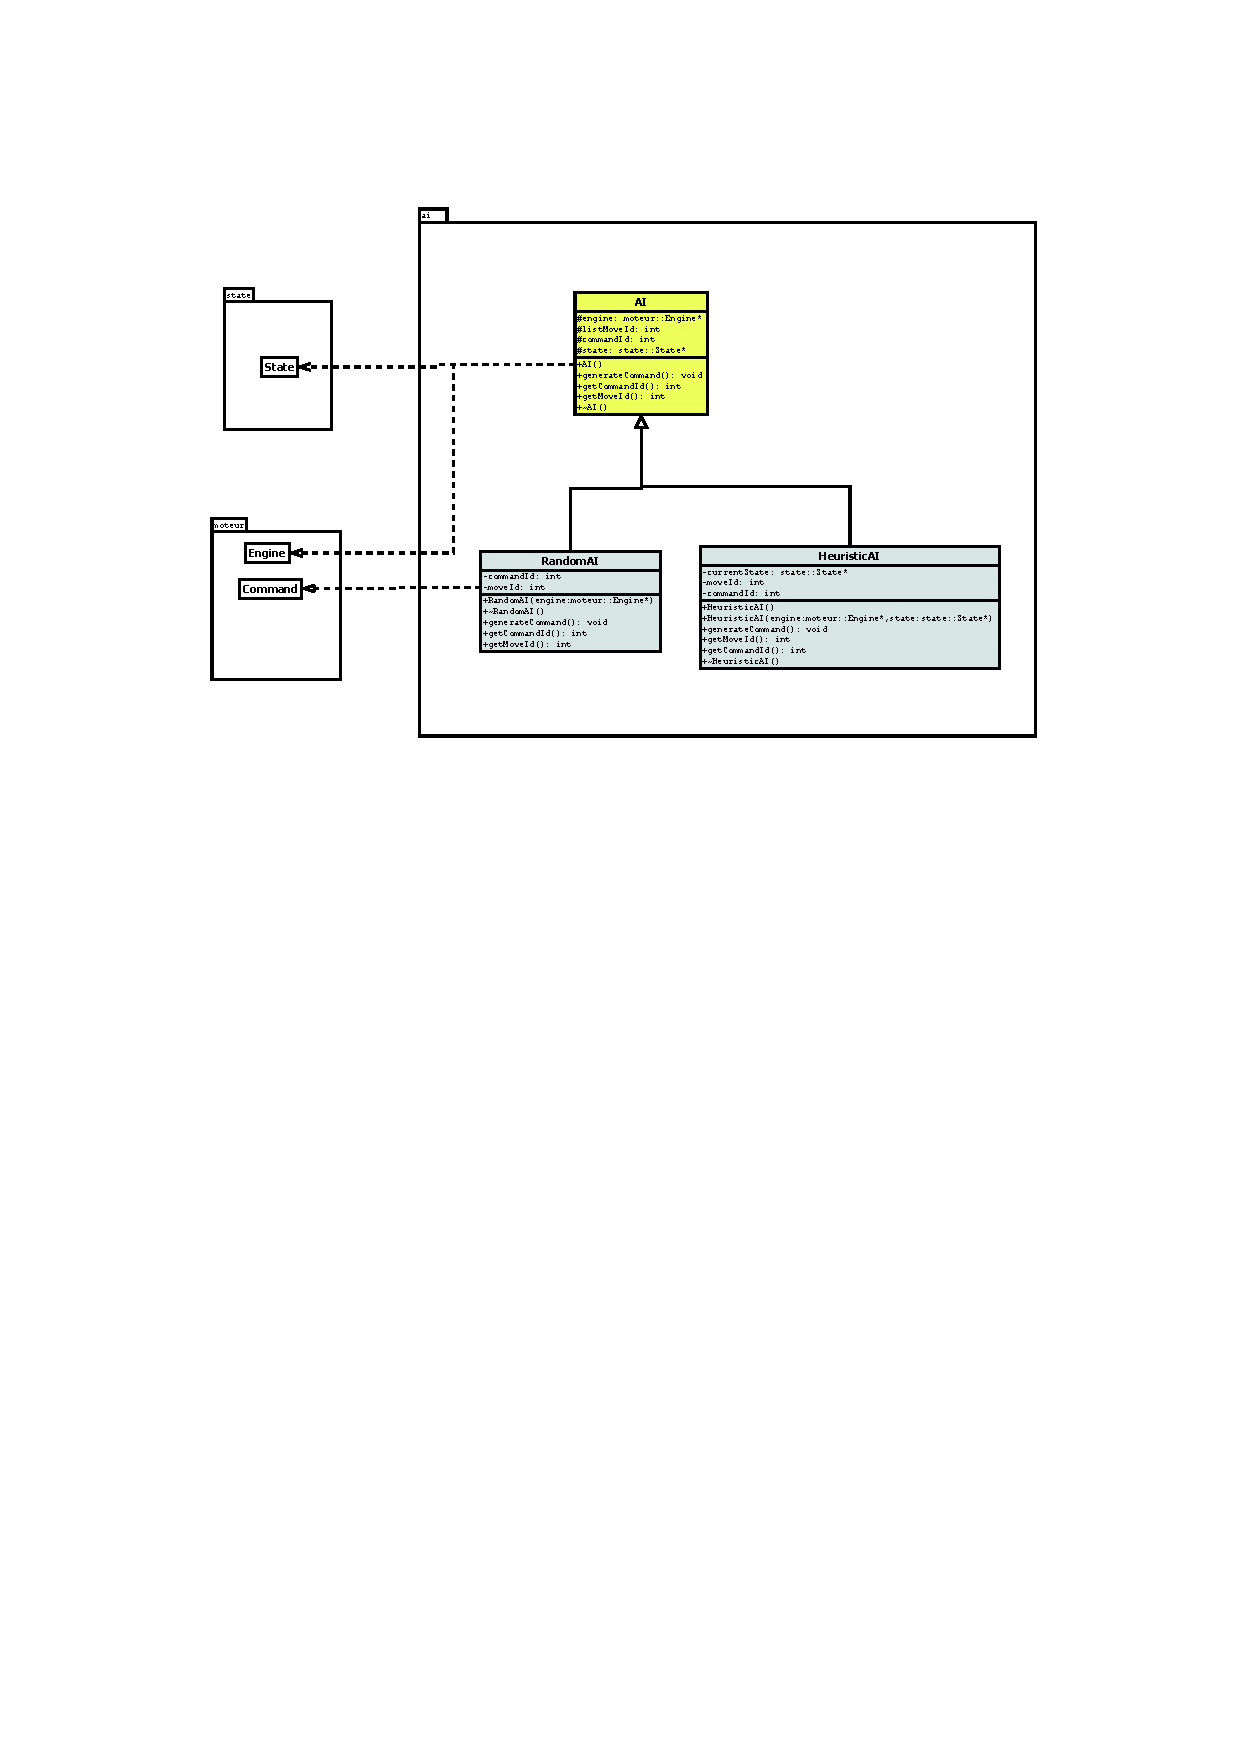
\includegraphics[width=0.9\paperheight]{ai.pdf}
%\caption{\label{uml:ai}Diagramme des classes d'intelligence artificielle.} 
%\end{figure}
%\end{landscape}


\section{Modularisation}
\label{sec:module}

\subsection{Organisation des modules}

\clearpage
\subsection{Conception logiciel}


%
%\begin{landscape}
%\begin{figure}[p]
%\includegraphics[width=0.9\paperheight]{module.pdf}
%\caption{\label{uml:module}Diagramme des classes pour la modularisation.} 
%\end{figure}
%\end{landscape}

\end{document}

